% !TEX program = pdflatex
\documentclass{beamer}

\usetheme{Boadilla}
\usepackage{graphicx}
\usepackage{hyperref}

\title{Early Diffusion Signals for Predicting Reach and Veracity in Social Media Rumor Cascades}
\subtitle{Paper track: thesis presentation}
\author{Jiahao Zhang}
\institute{University of Chicago}
\date{February 2026}

\begin{document}

\begin{frame}
\titlepage
% NOTES: Open with the core research theme and keep the framing concise. Transition quickly to the agenda.
\end{frame}

\begin{frame}{Outline}
\tableofcontents
% NOTES: Signal the flow: motivation, setup, results, implications, and next steps. Keep timing tight for a 5--10 minute talk.
\end{frame}

\section{Background}
\begin{frame}{Motivation \& Brief Literature}
\begin{itemize}
\item Early warning matters because diffusion often accelerates before verification catches up.
\item Prior studies find veracity-linked diffusion differences, but mostly from retrospective or full-cascade analysis.
\item Open gap: whether useful signals appear early enough to support actionable intervention.
\item Approach: early observation windows with structural and timing features beyond early volume alone.
\item Reported today: FibVID main results with Twitter15/16 retained as a benchmark comparison.
\end{itemize}
% NOTES: Anchor the talk on the timing problem and the methodological gap. End by stating exactly what evidence is shown today.
\end{frame}

\section{Data \& Methods}
\begin{frame}{Data}
\begin{itemize}
\item Main dataset: FibVID claim-level propagation records, converted into a cascade-compatible representation for the main analysis.
\item Comparative benchmark: Twitter15/16 rumor cascades in the original rumor-tree format.
\item Timestamps and propagation structure allow early-window evaluation without peeking at later spread.
\item The benchmark remains useful because it provides the clean native tree setting for the original pipeline.
\end{itemize}
% NOTES: Emphasize: this dataset uniquely supports early-window slicing and veracity supervision.
% NOTES: This deck now centers FibVID and uses Twitter15/16 as a benchmark comparison.
\end{frame}

\begin{frame}{Methods}
\begin{itemize}
\item Construct early observation windows from each cascade.
\item Extract structural and temporal features from partial trees.
\item Compare task-specific models under the same early-signal framework.
\item Evaluate whether early diffusion carries predictive information for both tasks.
\end{itemize}
\begin{center}
\IfFileExists{figs/early_window_tree.jpg}{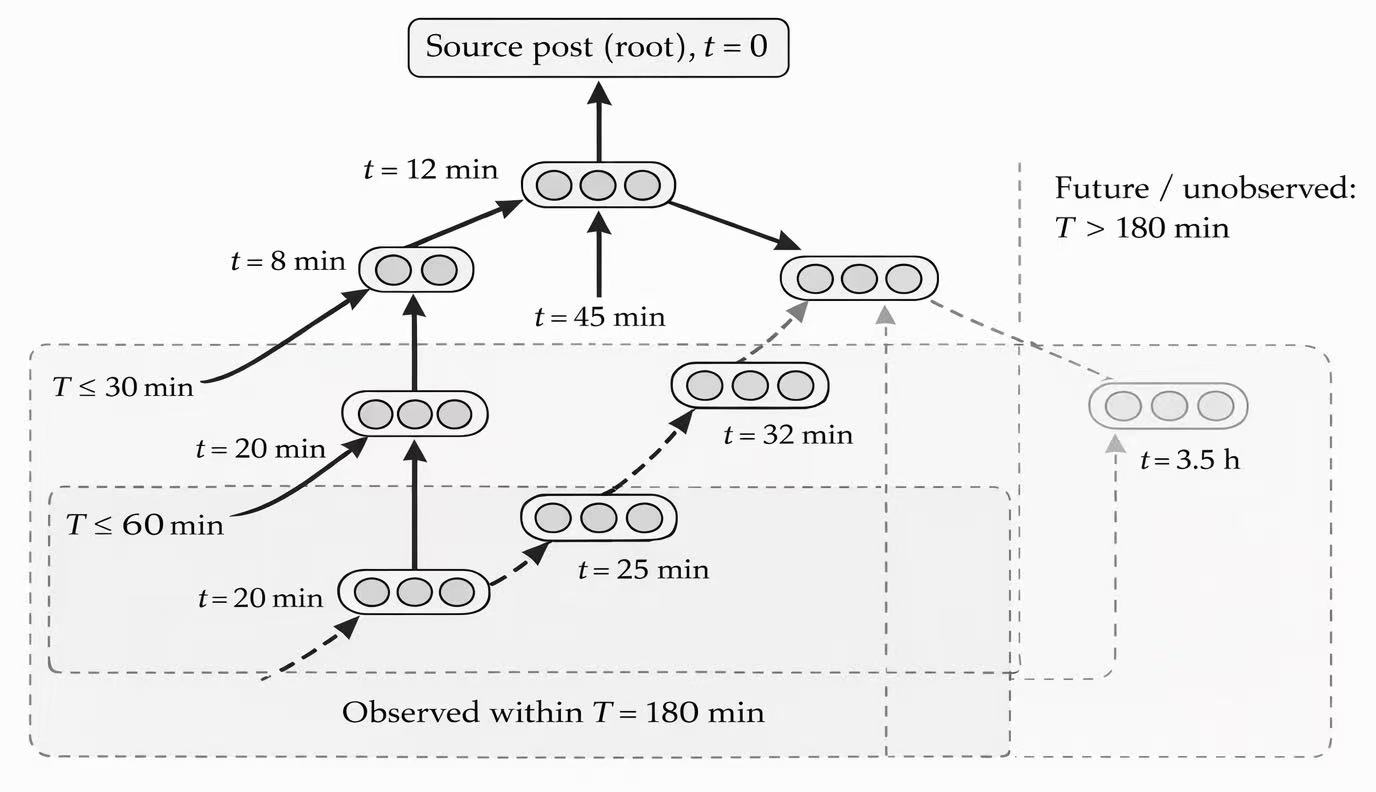
\includegraphics[width=0.72\linewidth]{figs/early_window_tree.jpg}}{\small (Missing file: figs/early_window_tree.jpg)}
\end{center}
% NOTES: Walk through pipeline steps once and point to the schematic. Avoid result interpretation on this slide.
\end{frame}

\section{Results}
\begin{frame}{Results (Twitter15/16): Veracity Prediction}
\begin{itemize}
\item Early-window diffusion features provide usable signal for veracity prediction.
\item The figure and table summarize previously generated Twitter15/16 veracity outputs.
\item Interpretation remains bounded to the current dataset and setup.
\end{itemize}
\begin{columns}[T,onlytextwidth]
\column{0.58\textwidth}
\centering
\IfFileExists{figs/F1K_k_veracity_primary.pdf}{
\includegraphics[width=0.95\linewidth]{figs/F1K_k_veracity_primary.pdf}}{\small (Missing file: figs/F1K_k_veracity_primary.pdf)}
\column{0.40\textwidth}
\IfFileExists{tables/twitter15_16_veracity_results.tex}{\centering
\small
\begin{tabular}{lcc}
\hline
Model & AUC (k=60) & SE \\
\hline
Logit & 0.640 & 0.014 \\
RF & 0.633 & 0.012 \\
XGBoost & 0.623 & 0.014 \\
\hline
\end{tabular}
}{\small (Missing file: tables/twitter15_16_veracity_results.tex)}
\end{columns}
% NOTES: Highlight the main directional takeaway without introducing new metrics. Keep language strictly tied to displayed outputs.
\end{frame}

\begin{frame}{Results (Twitter15/16): Reach Prediction}
\begin{itemize}
\item Early diffusion information is also informative for reach prediction.
\item The figure and table summarize previously generated Twitter15/16 reach outputs.
\item Together with veracity, this supports a multi-task early-signal perspective.
\end{itemize}
\begin{columns}[T,onlytextwidth]
\column{0.58\textwidth}
\centering
\IfFileExists{figs/F2K_k_reach_primary.pdf}{
\includegraphics[width=0.95\linewidth]{figs/F2K_k_reach_primary.pdf}}{\small (Missing file: figs/F2K_k_reach_primary.pdf)}
\column{0.40\textwidth}
\IfFileExists{tables/twitter15_16_reach_results.tex}{\centering
\small
\begin{tabular}{lcc}
\hline
Model & R\textsuperscript{2} (k=60) & SE \\
\hline
OLS & 0.254 & 0.054 \\
RFReg & 0.370 & 0.026 \\
XGBReg & 0.345 & 0.021 \\
\hline
\end{tabular}
}{\small (Missing file: tables/twitter15_16_reach_results.tex)}
\end{columns}
% NOTES: Keep comparison conceptual: same framework, different task. Avoid adding claims beyond the shown Twitter15/16 outputs.
\end{frame}

\section{Discussion}
\begin{frame}{Discussion}
\begin{itemize}
\item Practical use: supports earlier triage, monitoring priority, and resource allocation workflows.
\item Conceptual signal: early cascade structure appears informative beyond simple early volume counts.
\item Limitations: dataset and window-design choices may affect transferability and operational fit.
\item Risks to monitor: leakage pathways, heavy-tailed outcomes, and sensitivity to evaluation setup.
\end{itemize}
% NOTES: Balance practical implications with caution on limits. Frame this as evidence for utility, not a final deployment claim.
\end{frame}

\section{Next Steps}
\begin{frame}{Future Work}
\begin{itemize}
\item Time-window results are retained as the main robustness check.
\item Twitter15/16 now function as a benchmark rather than the only empirical setting.
\item A supplementary native-graph analysis on FibVID is used to check veracity sensitivity to representation.
\item The practical reading is staged prioritization, especially for likely high-impact cascades.
\end{itemize}
% NOTES: Mark all items as planned work and keep non-numeric. Position this as the roadmap after current Twitter15/16 findings.
\end{frame}

\section{Q\&A}
\begin{frame}{Q\&A + GitHub Repo}
\begin{itemize}
\item Code repository: \href{https://github.com/JiahaoZhang2001/Early-diffusion-signals}{github.com/JiahaoZhang2001/Early-diffusion-signals}
\item Questions?
\end{itemize}
% NOTES: Close with the repository link and invite discussion. Keep this slide minimal and readable.
\end{frame}

\end{document}
